\documentclass[12pt]{article}

% LaTeX packages
\usepackage{algorithm}
\usepackage{algorithmic}
\usepackage{amsmath}
\usepackage{amssymb}
\usepackage{amsthm}
\usepackage{fullpage}
\usepackage[colorlinks=true,citecolor=blue,linkcolor=blue]{hyperref}
\usepackage{natbib}
\usepackage{tikz}

% TikZ packages
\usetikzlibrary{arrows}
\usetikzlibrary{backgrounds}
\usetikzlibrary{calc}
\usetikzlibrary{cd}  % commutative diagrams
\usetikzlibrary{intersections}
\usetikzlibrary{patterns}
\usetikzlibrary{shapes}
\usetikzlibrary{through}

% Math environments
\newtheorem{definition}{Definition}
\newtheorem{proposition}[definition]{Proposition}
\newtheorem{lemma}[definition]{Lemma}
\newtheorem{theorem}[definition]{Theorem}
\newtheorem{corollary}[definition]{Corollary}

% Math symbols and commands
\newcommand{\R}{\mathbb{R}}  % set of real numbers
\newcommand{\indicator}[1]{\mathbf{1}\left[#1 \right]} % indicator
\newcommand{\ip}[2]{\left\langle #1, #2 \right\rangle} % inner product
\newcommand{\norm}[1]{\left\| #1 \right\|}  % norm of a vector or a matrix


\title{Online Multiclass Linear Classification with Bandit Feedback}

\author{
Alina Beygelzimer \and
D\'avid P\'al \and
Bal\'azs Sz\"or\'enyi \and
Devanathan Thiruvenkatachari \and
Chen-Yu Wei \and
Chicheng Zhang
}

\begin{document}

\maketitle

\begin{abstract}
TODO
\end{abstract}

\section{Introduction}
\label{section:introduction}

We study the online multiclass classification problem with bandit feedback. The
protocol of the problem is stated below. The problem was initially proposed by
\cite{Kakade-Shalev-Shwartz-Tewari-2008}. The corresponding problem with full
information feedback is solved by the classical \textsc{Multiclass Perceptron}
algorithm and its variants (see e.g.
\cite{Crammer-Dekel-Keshet-Shalev-Shwartz-Singer-2006}). The problem is quite
natural and potential applications include online advertising and online content
optimization where the feedback corresponds to a user's click.

\begin{algorithm}[h]
\caption{Online multiclass classification with bandit feedback
\label{algorithm:game-protocol}}
\begin{algorithmic}[1]
{
\REQUIRE{Number of classes $K$}
\FOR{$t=1,2,\dots$}
\STATE{Receive feature vector $x_t$}
\STATE{Environment \emph{secretly} chooses correct class label $y_t \in \{1,2,\dots,K\}$}
\STATE{Predict class label $\widehat y_t \in \{1,2,\dots,K\}$}
\STATE{Receive feedback $z_t \in \{0,1\}$ where $z_t = \begin{cases}
1 & \text{if $\widehat y_t = y_t$,} \\
0 & \text{if $\widehat y_t \neq y_t$.}
\end{cases}$
}
\ENDFOR
}
\end{algorithmic}
\end{algorithm}

In this paper, we focus on the special case when the examples are \emph{linearly
separable with a margin}. In the full-information feedback setting, it is well
know that if the examples have norm at most $R$ and are linearly separable with
a margin $\gamma$ then the \textsc{Multiclass Perceptron} algorithm makes at
most $(R/\gamma)^2$ mistakes. This result is very satisfactory since the upper
bound on the number of mistakes is information-theoretically optimal and at the
same time the \textsc{Multiclass Perceptron} algorithm has low time and memory
complexity.

The bandit feedback setting, however, is much more challenging. We start by
dissecting the notion of linear separability. We define two notions of linear
separability for multiclass classification: the standard linear separability
and \emph{strong linear separability}. For binary classification, these two
definitions are identical. However, they differ for multiclass classification.
For multiclass classification with $K$ classes the standard notion of linear
separability means that the examples from each class lie in an intersection of
$K-1$ halfspaces and the examples outside the class lie in the complement of the
intersection of the halfspaces. Strong linear separability means that examples
from each class can be separated from the remaining examples by a \emph{single}
hyperplane. We state the definitions precisely
in Section~\ref{section:notions-of-linear-separability}.

If the examples are strongly linearly separable, there is a simple and efficient
algorithm for the bandit feedback setting that makes at most $?/\gamma^2$
mistakes. The algorithm runs $K$ copies of the \textsc{Binary Perceptron}
algorithm.

For the standard notion of linear separability, we propose three algorithms with
various time-complexity-versus-mistake-bound trade-offs. Two of these algorithms
map the examples into a high-dimensional vector space induced by a kernel. In
this space the examples become \emph{strongly linearly separable}. This allows
us to run a kernelized version of the algorithm for the strongly linearly
separable case.

The two kernel-based algorithms differ by the choice of the kernel. The crux of
the problem is the analysis of the approximation properties of these kernels and
the way margin in original space under standard linear separability notion gets
transformed into a margin in the high-dimensional space under the strong
separability notion. This problem is related to the problem of learning
intersection of halfspaces and has been studied previously by
\cite{Klivans-Servedio-2008}.

The third algorithm is based on the obvious idea that two points that are close
enough must have the same label. Here, close enough means that they cannot be
separated from each other by a linear separator with a margin.

All three algorithms run in time that is polynomial in the dimension of the
feature vectors, the number of classes and the number of rounds. At the same
time, all three algorithms make number of mistakes that does \emph{not} depend
on the number of rounds. Instead, their number of mistakes depends only on the
margin, number of classes, dimension of the feature vectors, and the radius of
the ball in which the data lie.

Finally, we study two questions related to the computational and
information-theoretic hardness of the problem. Any algorithm for the bandit
setting collects information in the form of so called \emph{strongly labeled}
and \emph{weakly labeled} examples. Strongly-labeled examples are those for
which we know the class label. Weakly labeled example is an example for which we
know that class label can be anything except for a particular one class. First,
we show the offline problem of determining if a linear multiclass separator
exists for a set of strongly- and weakly-labeled examples is NP-complete. This
result is a simple consequence of the fact learning intersection of halfspaces
is NP-complete~\citep{Blum-Rivest-1993}. Second, we show that any algorithm that
uses only strongly-labeled examples and ignores weakly labeled examples makes at
least $\Omega(???)$ mistakes.


\section{Related work}
\label{section:related-work}

TODO


\section{Notions of linear separability}
\label{section:notions-of-linear-separability}

We define two notions of linear separability for multiclass classification. The
first notion is the standard notion of linear separability used in the proof of
mistake bound for the \textsc{Multiclass Perceptron} algorithm. The second
notion is stronger, i.e. more restrictive. However, it is more suitable for the
bandit setting, since it allows for a simple and efficient algorithm; see
Section~\ref{section:algorithm-for-strongly-linearly-separable-data}.

\begin{definition}
Let $(V,\ip{\cdot}{\cdot})$ be an inner product space, let $K$ be a positive
integer, and let $\gamma$ be a positive real number. Let $(x_1, y_1), (x_2,
y_2), \dots, (x_T, y_T)$ labeled examples in $V \times \{1,2,\dots,K\}$.

The examples are said to be \emph{linearly separable with a
margin $\gamma$} if there exist vectors $w_1, w_2, \dots, w_K \in V$ such
that
\begin{align}
\label{equation:linear-separability-1}
& \sum_{i=1}^K \norm{w_i}^2 \le 1 \; , \\
\label{equation:linear-separability-2}
& \forall t \in \{1,2,\dots,T\} \quad \forall i \in \{1,2,\dots, K\} \setminus \{y_t\} \qquad \qquad \ip{x_t}{w_{y_t}} \ge \ip{x_t}{w_i} + \gamma \; .
\end{align}

The examples are said to be \emph{strongly linearly separable with a
margin $\gamma$} if there exist vectors $w_1, w_2, \dots, w_K \in V$ such
that
\begin{align}
\label{equation:strong-linear-separability-1}
\forall i \in \{1,2,\dots,K\} \qquad \qquad \norm{w_i}^2 & \le 1 \; , \\
\label{equation:strong-linear-separability-2}
\forall t \in \{1,2,\dots,T\} \qquad \qquad \ip{x_t}{w_{y_t}} &\ge \gamma \; , \\
\label{equation:strong-linear-separability-3}
\forall t \in \{1,2,\dots,T\} \qquad \forall i \in \{1,2,\dots, K\} \setminus \{y_t\} \qquad \qquad \ip{x_t}{w_i} & \le - \gamma \; .
\end{align}
\end{definition}

It is easy to see that if labeled examples are strongly linearly
separable with margin $\gamma$ then they are linearly separable with margin
$2\gamma/\sqrt{K}$. Indeed, if $w_1, w_2, \dots, w_K \in V$
satisfy \eqref{equation:strong-linear-separability-1},
\eqref{equation:strong-linear-separability-2},
\eqref{equation:strong-linear-separability-3} then $w_1' = w_1/\sqrt{K}, w_2' =
w_2/\sqrt{K}, \dots, w_K' = w_K/\sqrt{K}$ satisfy
\eqref{equation:linear-separability-1} and
\eqref{equation:linear-separability-2} with margin $\gamma' = 2\gamma/\sqrt{K}$.

Similarly, if $K=2$ and labeled examples are linearly separable with a margin
$\gamma$ then they are strongly linearly separable with the same margin
$\gamma$. Indeed, if $w_1, w_2$ satisfy \eqref{equation:linear-separability-1}
and \eqref{equation:linear-separability-2} then $w_1' = w_1 - w_2$ and $w_2' =
w_2 - w_1$ satisfy \eqref{equation:strong-linear-separability-1},
\eqref{equation:strong-linear-separability-2},
\eqref{equation:strong-linear-separability-3}.

However, if $K=3$ there exists a set of labeled examples in an inner product
space that is linearly separable with a positive margin $\gamma$ but it is not
strongly linearly separable for any positive $\gamma$. This is best illustrated
on Figure~\ref{figure:linearly-separable-examples-with-margin}.

\begin{figure}
\begin{center}
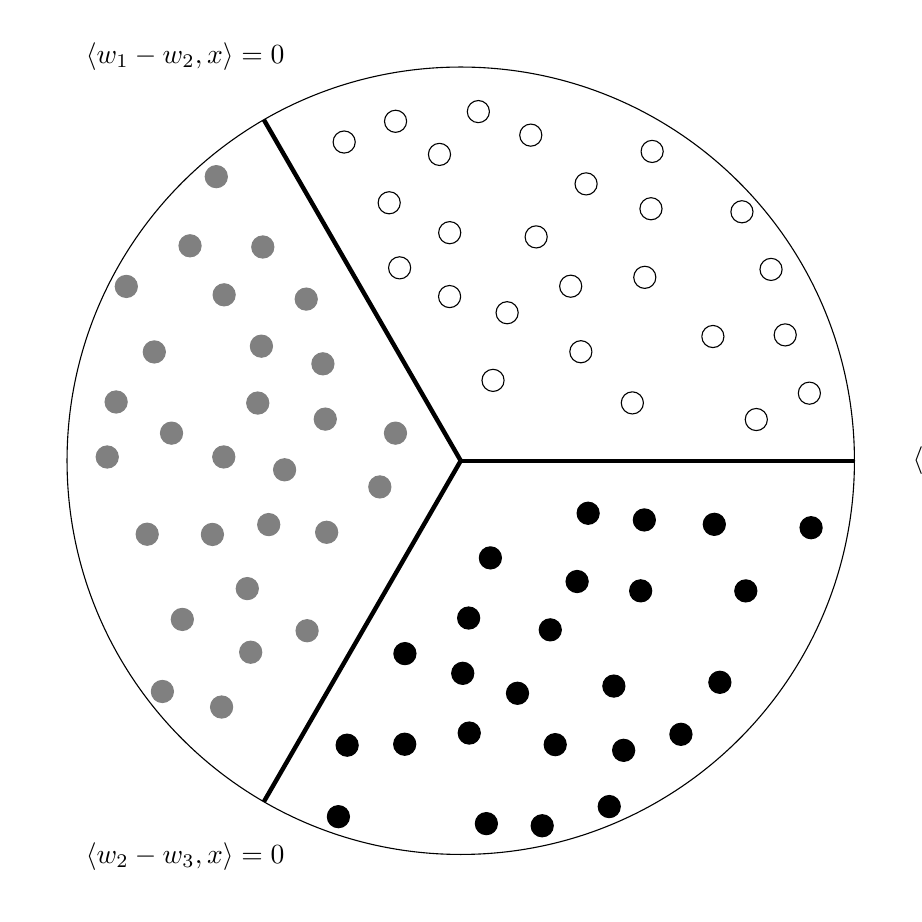
\begin{tikzpicture}

  \useasboundingbox (-5.5,-5.5) rectangle (5.5,5.5);
  % \draw[help lines] (-5.5,-5.5) rectangle (5.5,5.5);

  % Grid and coordinate axes
  %% \draw[help lines] (-5.2,-5.2) grid (5.2,5.2);
  %% \draw[thick, ->, >=latex] (-5.2,0) -- (5.2,0);
  %% \draw[thick, ->,  >=latex] (0,-5.2) -- (0,5.2);

  % Notable points
  \coordinate (Origin) at (0,0);

  \coordinate [label={[xshift=-10mm, yshift=5mm]$\ip{w_1 - w_2}{x} = 0$}] (A) at (120:5);
  \coordinate [label={[xshift=-10mm, yshift=-10mm]$\ip{w_2 - w_3}{x} = 0$}] (B) at (240:5);
  \coordinate [label={[xshift=+20mm, yshift=-3mm]$\ip{w_3 - w_1}{x} = 0$}] (C) at (360:5);

  % Circle which contains all the examples.
  \draw (Origin) circle (5);

  \draw[ultra thick] (Origin) -- (A);
  \draw[ultra thick] (Origin) -- (B);
  \draw[ultra thick] (Origin) -- (C);

  % Class 0 points. Angles between 0.0 and 120.0
  \draw[color=black, fill=none]
                    (7.94:3.79) circle (4pt)
                    (10.97:4.51) circle (4pt)
                    (18.63:2.30) circle (4pt)
                    (21.20:4.42) circle (4pt)
                    (26.23:3.57) circle (4pt)
                    (31.66:4.63) circle (4pt)
                    (41.52:4.77) circle (4pt)
                    (42.22:2.06) circle (4pt)
                    (44.90:3.30) circle (4pt)
                    (52.95:4.01) circle (4pt)
                    (57.79:2.62) circle (4pt)
                    (58.25:4.62) circle (4pt)
                    (65.64:3.86) circle (4pt)
                    (68.11:1.10) circle (4pt)
                    (71.38:3.00) circle (4pt)
                    (72.60:1.97) circle (4pt)
                    (77.86:4.23) circle (4pt)
                    (87.11:4.44) circle (4pt)
                    (92.77:2.90) circle (4pt)
                    (93.88:2.09) circle (4pt)
                    (93.97:3.90) circle (4pt)
                    (100.87:4.39) circle (4pt)
                    (105.50:3.40) circle (4pt)
                    (107.58:2.57) circle (4pt)
                    (110.09:4.31) circle (4pt)
                    ;

  % Class 1 points. Angles between 120.0 and 240.0
  \draw[color=gray, fill=gray]
                    (130.71:4.76) circle (4pt)
                    (132.80:3.70) circle (4pt)
                    (133.71:2.84) circle (4pt)
                    (141.55:4.39) circle (4pt)
                    (144.89:2.14) circle (4pt)
                    (144.96:3.67) circle (4pt)
                    (150.11:2.92) circle (4pt)
                    (152.47:4.79) circle (4pt)
                    (157.09:0.90) circle (4pt)
                    (160.45:4.13) circle (4pt)
                    (162.92:1.80) circle (4pt)
                    (164.13:2.68) circle (4pt)
                    (170.32:4.44) circle (4pt)
                    (174.55:3.69) circle (4pt)
                    (179.08:3.01) circle (4pt)
                    (179.39:4.49) circle (4pt)
                    (182.94:2.24) circle (4pt)
                    (193.19:4.09) circle (4pt)
                    (196.53:3.29) circle (4pt)
                    (197.93:1.08) circle (4pt)
                    (198.39:2.57) circle (4pt)
                    (208.08:1.93) circle (4pt)
                    (209.68:4.07) circle (4pt)
                    (210.92:3.16) circle (4pt)
                    (217.72:4.79) circle (4pt)
                    (222.35:3.61) circle (4pt)
                    (225.84:4.36) circle (4pt)
                    (227.89:2.91) circle (4pt)
                    ;

% Class 2 points. Angles between 240.0 and 360.0
  \draw[color=black, fill=black]
                    (248.23:3.89) circle (4pt)
                    (251.03:4.78) circle (4pt)
                    (253.86:2.55) circle (4pt)
                    (258.82:3.67) circle (4pt)
                    (270.54:2.70) circle (4pt)
                    (271.79:3.46) circle (4pt)
                    (272.88:2.00) circle (4pt)
                    (274.04:4.62) circle (4pt)
                    (282.58:4.75) circle (4pt)
                    (283.72:3.04) circle (4pt)
                    (286.97:1.29) circle (4pt)
                    (288.41:3.80) circle (4pt)
                    (293.24:4.78) circle (4pt)
                    (297.90:2.43) circle (4pt)
                    (299.36:4.22) circle (4pt)
                    (304.20:3.46) circle (4pt)
                    (308.83:4.46) circle (4pt)
                    (313.94:2.13) circle (4pt)
                    (319.47:4.33) circle (4pt)
                    (324.13:2.82) circle (4pt)
                    (335.46:3.98) circle (4pt)
                    (337.60:1.75) circle (4pt)
                    (342.13:2.45) circle (4pt)
                    (345.92:3.32) circle (4pt)
                    (349.18:4.53) circle (4pt)
                    ;

\end{tikzpicture}

\end{center}
\caption{The figure shows labeled examples in $\R^2$. There are $K=3$ classes. The
examples of each class are colored white, gray and black respectively. All
examples lie in the ball of radius $R$ centered at the origin. While the
examples are linearly separable with a positive margin $\gamma$, they are
\emph{not} strongly linearly separable for any positive margin $\gamma$,
however.
}
\label{figure:linearly-separable-examples-with-margin}
\end{figure}

\section{Algorithm for strongly linearly separable data}
\label{section:algorithm-for-strongly-linearly-separable-data}

\begin{algorithm}[h]
\caption{Algorithm for strongly linearly separable examples
\label{algorithm:algorithm-for-strongly-linearly-separable-examples}}
\begin{algorithmic}[1]
{
\REQUIRE{Number of classes $K$}
\STATE{Initialize $w_1^{(1)} = w_2^{(1)} = \dots = w_K^{(1)} = 0$}
\FOR{$t=1,2,\dots$}
\STATE{Receive feature vector $x_t$}
\STATE{Compute $S_t = \{ i ~:~ \ip{w_i^{(t)}}{x_t} > 0 \}$}
\IF{$|S_t| = 1$}
\STATE{Predict $\widehat y_t$ where $\widehat y_t \in S_t$}
\ELSE
\STATE{Predict $\widehat y_t \sim \text{Uniform}(\{1,2,\dots,K\})$}
\ENDIF
\STATE{Receive feedback $z_t \in \{0,1\}$ where $z_t = \indicator{\widehat y_t = y_t}$}
\STATE{Update $w_i^{(t+1)} = w_i^{(t)}$ for all $i \in \{1,2,\dots,K\} \setminus \{\widehat y_t\}$}
\IF{$z_t = 0$}
\STATE{Update $w_{\widehat y_t}^{(t+1)} = w_{\widehat y_t}^{(t)} - x_t$}
\ELSE
\STATE{Update $w_{\widehat y_t}^{(t+1)} = w_{\widehat y_t}^{(t)}$}
\ENDIF
\ENDFOR
}
\end{algorithmic}
\end{algorithm}

\begin{theorem}
Let $(V, \ip{\cdot}{\cdot})$ be any inner product space, let $K$ be a positive
integer, $\gamma$ a positive real number, $R$ be a non-negative real number
If $(x_1, y_1), (x_2, y_2), \dots, (x_T, y_T)$ is a sequence of labeled examples
in $V \times \{1,2,\dots,K\}$ such that the examples are strongly separable with
margin $\gamma$ and $\norm{x_1}, \norm{x_2}, \dots, \norm{x_T} \le R$ then
Algorithm~\ref{algorithm:algorithm-for-strongly-linearly-separable-examples}
makes at most $K (R/\gamma)^2$ mistakes.
\end{theorem}

\begin{proof}
TODO
\end{proof}


\section{Converting linear separability to strong linear separability}

TODO


\section{Nearest neighbor algorithm}

TODO


\section{NP-hardness of the weak labeling problem}

TODO


\section{Mistake lower bound for ignorant algorithms}

TODO



\bibliographystyle{plainnat}
\bibliography{biblio}

\end{document}
